\chapter{Entropy, Surprisal, and the Shannon Limit}
\label{ch:entropy}

\section{The Architecture of Uncertainty}

Before we can ask how a deep neural network learns to represent the world, we must first ask what it means to represent anything at all. When a vision model classifies an image as a dog, or a language model predicts the next word in a sentence, it is fundamentally resolving uncertainty. It begins in a state of ignorance---any image could theoretically be any class---and, through the processing of data, collapses that vast space of possibilities down to a single, highly probable conclusion. 

To make this process mathematically tractable, we need a formal currency for uncertainty. We need to be able to measure exactly how much ``surprise'' is contained in an event, and by extension, how much uncertainty is resolved when that event is observed. This is the bedrock of information theory, first laid down by Claude Shannon in his 1948 landmark paper \cite{shannon1948mathematical}. Shannon recognized that the semantic meaning of a message---whether it is a profound poem or a trivial string of digits---is irrelevant to the engineering problem of transmitting it. What matters is predictability.

Imagine a heavily biased weather system where every day is sunny. If a meteorologist tells you tomorrow will be sunny, you have learned almost nothing. Your internal model of the world remains unchanged. The message carries very little information. But if the meteorologist tells you it will snow in the middle of July, you are highly surprised. This event forces a massive update to your internal model. The message carries a tremendous amount of information. Information, therefore, is inversely related to probability. The less likely an event is, the more information it contains when it occurs.

We call this inherent informational value \textit{surprisal}. When we average this surprisal over all possible events in a system, we arrive at the system's \textit{entropy}. Entropy is a measure of the average uncertainty, or the expected amount of information, inherent in the variable's possible outcomes. It is the minimum number of bits needed, on average, to encode a sequence of symbols drawn from that distribution. 

In the context of deep learning, entropy is the invisible floor beneath all our architectures. When we train a generative model to synthesize realistic images, we are fundamentally trying to approximate the entropy of the natural image manifold. When we compress a high-dimensional input into a low-dimensional latent vector $z$, we are squeezing the data through a channel whose capacity is bounded by the laws of information theory. Before we can optimize the weights of a neural network $f_\theta$, we must understand the theoretical limits of the representations it builds.

\section{Mathematical Formulation}

We formalize the intuition of surprisal by defining it mathematically. Let $X$ be a discrete random variable taking values $x$ in an alphabet $\mathcal{X}$, with probability mass function $p(x) = \text{Pr}(X = x)$.

\begin{definition}[Surprisal / Self-Information]
The surprisal of an event $x$ with probability $p(x)$ is defined as:
\begin{equation}
    I(x) = -\log p(x)
\end{equation}
When the logarithm is base 2, the unit of surprisal is the \textit{bit}. If the natural logarithm is used, the unit is the \textit{nat}.
\end{definition}

This definition perfectly captures our intuition: if $p(x) = 1$, the surprisal is $-\log(1) = 0$. If $p(x)$ approaches 0, the surprisal approaches infinity. Furthermore, for two independent events $x$ and $y$, their joint probability is $p(x,y) = p(x)p(y)$. The surprisal of observing both is $I(x,y) = -\log(p(x)p(y)) = -\log p(x) - \log p(y) = I(x) + I(y)$. Information is additive.

\begin{definition}[Shannon Entropy]
The Shannon entropy $H(X)$ of a discrete random variable $X$ is the expected value of the surprisal of its outcomes:
\begin{equation}
    H(X) = \mathbb{E}_{x \sim p}[-\log p(x)] = -\sum_{x \in \mathcal{X}} p(x) \log p(x)
\end{equation}
By convention, we define $0 \log 0 = 0$, consistent with the limit $\lim_{p \to 0} p \log p = 0$.
\end{definition}

\subsection{Properties of Entropy}

For a binary random variable $X$ where $P(X=1) = p$ and $P(X=0) = 1-p$, the entropy is known as the binary entropy function, denoted $H(p)$.
\begin{equation}
    H(p) = -p \log_2 p - (1-p) \log_2 (1-p)
\end{equation}

\begin{figure}[ht]
    \centering
    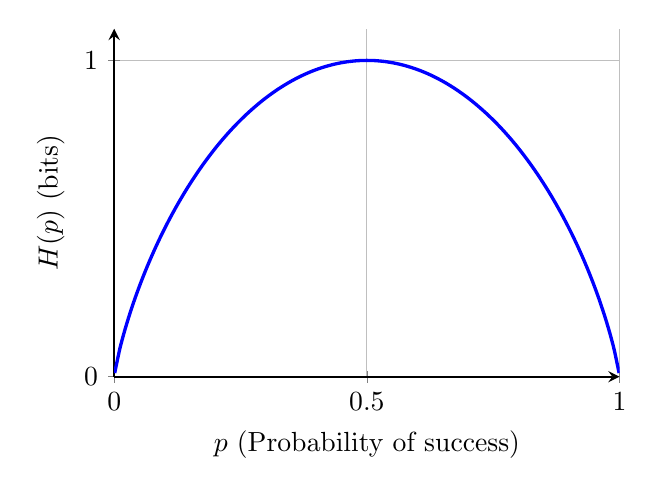
\begin{tikzpicture}
        \begin{axis}[
            width=8cm, height=6cm,
            xlabel={$p$ (Probability of success)},
            ylabel={$H(p)$ (bits)},
            xmin=0, xmax=1,
            ymin=0, ymax=1.1,
            xtick={0, 0.5, 1},
            ytick={0, 1},
            grid=major,
            axis lines=left,
            thick,
            smooth
        ]
        \addplot[domain=0.001:0.999, samples=100, blue, very thick] 
            {-x*log2(x) - (1-x)*log2(1-x)};
        \end{axis}
    \end{tikzpicture}
    \caption{The binary entropy function $H(p)$. Uncertainty is maximized when $p=0.5$ (a fair coin), yielding 1 bit of entropy.}
    \label{fig:binary_entropy}
\end{figure}

As seen in Figure~\ref{fig:binary_entropy}, entropy is maximized when the distribution is uniform (maximum uncertainty) and minimized when the distribution is deterministic (zero uncertainty).

\begin{theorem}[Maximum Entropy for Discrete Variables]
\label{thm:max_entropy}
For a discrete random variable $X$ with an alphabet size $|\mathcal{X}|$, the entropy $H(X)$ satisfies:
\begin{equation}
    0 \leq H(X) \leq \log |\mathcal{X}|
\end{equation}
The upper bound is achieved if and only if $X$ is uniformly distributed over $\mathcal{X}$.
\end{theorem}

\begin{proof}
Let $p(x)$ be the probability distribution of $X$, and let $u(x) = 1/|\mathcal{X}|$ be the uniform distribution. We use the fundamental inequality $\ln z \leq z - 1$ for $z > 0$, with equality if and only if $z = 1$.
\begin{align*}
    H(X) - \log |\mathcal{X}| &= \sum_{x} p(x) \log \frac{1}{p(x)} - \sum_{x} p(x) \log |\mathcal{X}| \\
    &= \sum_{x} p(x) \log \frac{1}{p(x)|\mathcal{X}|} \\
    &= \frac{1}{\ln 2} \sum_{x} p(x) \ln \frac{u(x)}{p(x)} \\
    &\leq \frac{1}{\ln 2} \sum_{x} p(x) \left( \frac{u(x)}{p(x)} - 1 \right) \\
    &= \frac{1}{\ln 2} \left( \sum_{x} u(x) - \sum_{x} p(x) \right) \\
    &= \frac{1}{\ln 2} (1 - 1) = 0
\end{align*}
Equality holds if and only if $u(x)/p(x) = 1$ for all $x$, meaning $p(x) = 1/|\mathcal{X}|$.
\end{proof}

\subsection{Shannon's Source Coding Theorem}

Why is $H(X)$ the fundamental limit of compression? Shannon's Source Coding Theorem establishes that $H(X)$ is the minimum expected length of any uniquely decodable binary code for $X$. 

Let $C(x)$ be the codeword for symbol $x$, and $l(x)$ be its length in bits. The expected length of the code is $L = \sum_x p(x) l(x)$.

\begin{theorem}[Shannon's Source Coding Theorem (Noiseless)]
\label{thm:source_coding}
For any uniquely decodable code representing a discrete random variable $X$, the expected length $L$ is bounded by:
\begin{equation}
    L \geq H(X)
\end{equation}
Furthermore, there exists a prefix code such that $L < H(X) + 1$.
\end{theorem}
The proof relies on the Kraft-McMillan inequality ($\sum_x 2^{-l(x)} \leq 1$), which dictates the lengths of prefix-free codes \cite{cover1999elements}.

\subsection{Worked Numerical Example}

Consider a simple weather prediction model that categorizes the next day into four states $\mathcal{X} = \{\text{Sunny, Cloudy, Rainy, Snowy}\}$ with probabilities $p = \{0.5, 0.25, 0.125, 0.125\}$.

First, we compute the Shannon entropy $H(X)$:
\begin{align*}
    H(X) &= - \left( 0.5 \log_2 0.5 + 0.25 \log_2 0.25 + 0.125 \log_2 0.125 + 0.125 \log_2 0.125 \right) \\
    &= 0.5(1) + 0.25(2) + 0.125(3) + 0.125(3) \\
    &= 0.5 + 0.5 + 0.375 + 0.375 \\
    &= 1.75 \text{ bits}
\end{align*}

To achieve a code length that matches this theoretical minimum, we can construct a Huffman tree (Figure~\ref{fig:huffman}). We assign shorter codewords to more frequent events.

\begin{figure}[ht]
    \centering
    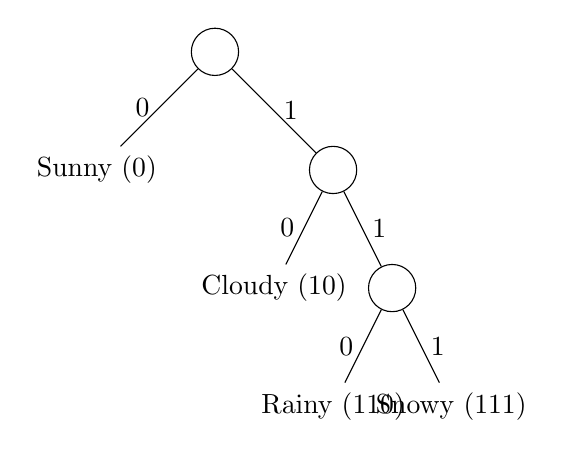
\begin{tikzpicture}[level distance=1.5cm,
      level 1/.style={sibling distance=3cm},
      level 2/.style={sibling distance=1.5cm},
      level 3/.style={sibling distance=1.5cm},
      circle node/.style={circle,draw,minimum size=6mm,inner sep=0pt}]
      
      \node[circle node] {}
        child {node {Sunny (0)} edge from parent node[left,draw=none] {0}}
        child {node[circle node] {}
          child {node {Cloudy (10)} edge from parent node[left,draw=none] {0}}
          child {node[circle node] {}
            child {node {Rainy (110)} edge from parent node[left,draw=none] {0}}
            child {node {Snowy (111)} edge from parent node[right,draw=none] {1}}
            edge from parent node[right,draw=none] {1}
          }
          edge from parent node[right,draw=none] {1}
        };
    \end{tikzpicture}
    \caption{Huffman tree for the weather prediction example. The expected code length $L = 0.5(1) + 0.25(2) + 0.125(3) + 0.125(3) = 1.75$ bits, perfectly matching $H(X)$.}
    \label{fig:huffman}
\end{figure}

In this ideal scenario, the expected code length $L$ exactly equals $H(X)$, because all probabilities are negative powers of 2. In deep learning, neural networks essentially perform a continuous version of this coding, mapping dense raw inputs into compressed latent codes $z$. 

\begin{horizon}
While Shannon's theorems strictly govern discrete, stationary distributions, the data processed by deep neural networks is often continuous, non-stationary, and intrinsically high-dimensional. Classical entropy assumes a known probability distribution $P$, but a neural network $f_\theta$ only ever sees empirical samples from a finite dataset $\mathcal{D}$. 

It is conjectured that for highly overparameterized models, the implicit regularization of stochastic gradient descent operates by minimizing a localized, empirical form of entropy over the parameter manifold. Under this view, the network does not merely compress the input; it actively reshapes the alphabet $\mathcal{X}$ into an internal latent geometry $\mathcal{Z}$ where the source coding bounds are continuously re-negotiated during training. 

An open question is whether the fundamental limits of the Source Coding Theorem can be meaningfully translated into a "Representation Coding Theorem" for intermediate layers of deep networks. If the latent space dynamically adapts, what serves as the true capacity limit? Future work in the intersection of information bottleneck theory and learning dynamics might reveal that neural networks naturally converge to solutions that are optimal not just for generalization, but for thermodynamic efficiency.
\end{horizon}

\section*{Summary}
In this chapter, we introduced the foundational currency of information theory: surprisal. By averaging surprisal across a probability distribution, we defined Shannon entropy $H(X)$, which quantifies the average uncertainty of a random variable. We proved that uniform distributions maximize entropy, establishing a ceiling on uncertainty. Through Shannon's Source Coding Theorem, we demonstrated that $H(X)$ represents the absolute theoretical limit for lossless data compression, setting the stage for how neural networks compress and encode representations.

\section*{Exercises}
\begin{enumerate}
    \item \textbf{Calculating Entropy:} Let $X$ represent the roll of a loaded six-sided die where $p(1)=p(2)=p(3)=p(4)=1/8$ and $p(5)=p(6)=1/4$. Calculate the Shannon entropy $H(X)$ in bits.
    \item \textbf{Binary Source:} A source produces a binary sequence of $1$s and $0$s. The probability of a $1$ is $p$. Plot the entropy $H(p)$ and find the value of $p$ that maximizes it using calculus.
    \item \textbf{Infinite Alphabet:} Consider a geometric random variable $X$ with probability mass function $p(k) = (1-p)^{k-1}p$ for $k = 1, 2, 3, \dots$. Derive a closed-form expression for the entropy $H(X)$. 
    \item \textbf{Network Weights:} Suppose a highly quantized neural network has $10^6$ parameters, each taking one of three values $\{-1, 0, 1\}$ with probabilities $\{0.2, 0.6, 0.2\}$. What is the minimum theoretical file size (in bytes) required to store these weights losslessly?
    \item \textbf{Empirical vs True Entropy:} Discuss the difficulty of estimating the entropy of an image dataset (e.g., $256 \times 256$ RGB images) directly from its empirical distribution $\mathcal{D}$. Why does the plug-in estimator $\hat{H} = -\sum \hat{p}(x)\log \hat{p}(x)$ fail catastrophically in this high-dimensional regime?
\end{enumerate}
